\documentclass[a4paper]{scrreprt}
\usepackage{graphicx,picture}
\title{Eccentricity Matters}
% \author{Muhammad Zeeshan}
% \date{\today}

\begin{document}
%\maketitle

\section{Third Report of the Referee -- DS13372}

The added paragraph does not solve major concern 1 that I have raised.
It only states that the eccentricity is defined at 10 Hz. But the
errors on the measurements of chirp mass are drawn from the
distributions with parameter $\beta$ fitted with velocity $(v = (\pi
M_c^{e} f)^{1/3})$ corresponding to reference frequency of $20 Hz$
which is a function of eccentric chirp mass for EBBH. But the $M_c^{e}$
is defined at $10 Hz$ as per the eccentricity.

All this makes measurement of $M_c^{e}$ and related error inconsistent.
I recommend using errors on $M_c$ and $M_c^{e}$ do be drawn using $\beta$
defined at $f = 10 Hz$ and rerunning the analysis assuming parameter
estimation is done with the reference frequency of $10 Hz$.

\section{Third Response to the Referee -- DS13372}


We have resubmitted an unchanged manuscript.  We respectfully disagree with the referee's request, for reasons described
below.  In brief, the revised calculation does not qualitatively change our conclusions; conversely, we think the
request reflects a misunderstanding of our modeling approach, and any requested change would perpetuate this confusion
among other readers.
However, if the editor concurs with the referee's request, we have performed the requested revised calculation,
described below.

\begin{itemize}

    \item \emph{$M_c$ uncertainty does not evolve (within our approximation)}:
We employ uncorrelated synthetic measurement errors for each parameter, whose covariance does not change with eccentricity.  In particular, the assumed chirp mass error is defined by Eq. 12.  While the reference eccentricity does
depend on the choice of reference frequency for eccentricity, the parameters entering into Eq. 12 do not: they only depend on binary masses. Therefore, we have no mechanism which changes our adopted uncertainty model that depends on the frequency at
which the eccentricity.
Since we assume uncorrelated measurement errors in $M_c$, $\eta$, and eccentricity which do not depend on eccentricity, these measurement errors must furthermore agree with conventional estimates for the zero-eccentricity measurement error
for $M_c$, $\eta$.  The choices described in our draft for these uncertainties $\Sigma_{ab}$ for $a,b ={M_c,\eta}$ are conventional.
The measurement error for $M_c$ does depend on $M_c$ and the most \textbf{sensitive frequencies} to which a detector is
sensitive (if inspiral-dominated). The actual (correlated) dependence of $M_c$ measurement error on binary parameters is
complicated, particularly since some of the signals involved are not inspiral-dominated. For this reason, following
previous work, we have \textbf{conservatively} used an \textbf{estimate} that depends on a \textbf{lower frequency}.  This model specifically
\textbf{overstates} our uncertainty in chirp mass, while producing qualitatively similar synthetic posterior distributions.

The chirp mass is not convention-dependent and does not evolve with frequency.  Its measurement uncertainty is therefore independent of the choice of the \textbf{arbitrary} reference frequency used to specify waveform initial conditions
like spin and eccentricity.   

The appearance of a quantity with frequency units in our expression for $\beta$ does not have any relationship to the
initial conditions used to specify waveform parameters like precessing spins or eccentricity.  It is simply an
calibrated, empirical, and extremely conservative estimate of how well contemporary gravitational wave detectors might measure chirp masses.

    \item \emph{Systematics larger than requested effect}:
As in previous comparable studies, we employ synthetic estimates for parameter inference accuracy.  
These synthetic estimates are never exact representations of real end-to-end data analysis.  Moreover, even realistic data
analysis has substantial systematic uncertainty (e.g,. waveform modeling) and arbitrary analysis choices (e.g., the
lower frequency used in inference, the reference PSD in a synthetic study, et cetera).     

 In our opinion, the referee is asking for a reanalysis changing an assumption that is well below the systematic uncertainties involved
in our proof-of-concept demonstration. However, we have \textbf{provided the re-analysis} below for the referee's convenience to demonstrate that the requested change does not affect our results.
\end{itemize}


We have generated the new injections as recommended by the referee given in Fig. \ref{fig:fig0}.  We note that
\textbf{no reference frequency appears in the algorithm} used to generate these injections : the injections are drawn from the identical
distribution as our original set.
\begin{figure}[h]
    \centering
    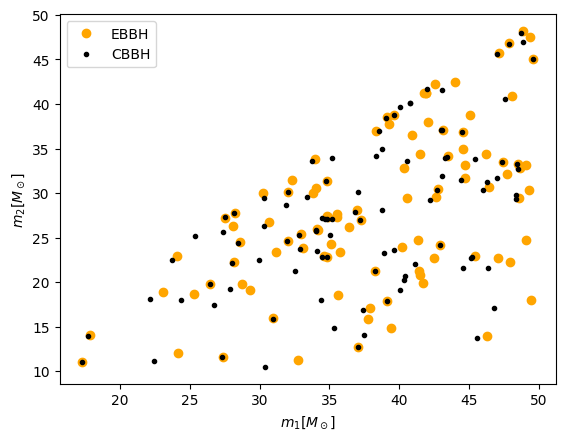
\includegraphics[width=0.49\textwidth]{figures/pop2d_0.05.png}
    \caption{Injections}
    \label{fig:fig0}
\end{figure}

The Fig. \ref{fig:fig1} show the comparison of the posteriors associated with the new injections requested by the
referee, using two approaches: first,  choosing the chirp mass error parameter $\beta$ with the same fiducial frequency
scale used in draft ($f=20 Hz$), and second repeating this calculation but using a lower fiducial frequency scale ($f=10 Hz$).

\begin{figure}[h]
    \centering
    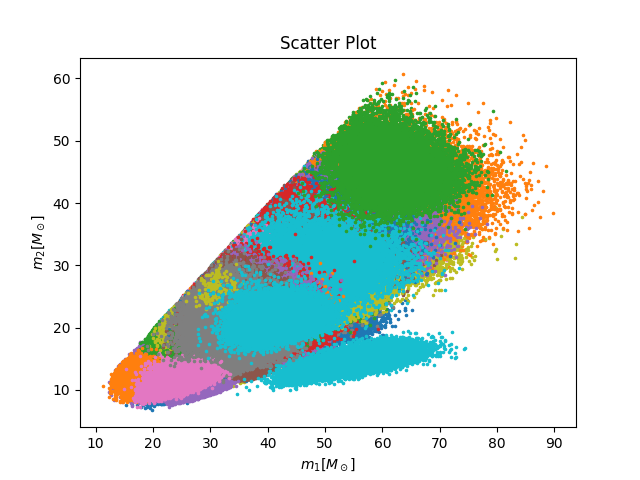
\includegraphics[width=0.49\textwidth]{figures/scatter_plot.png}
    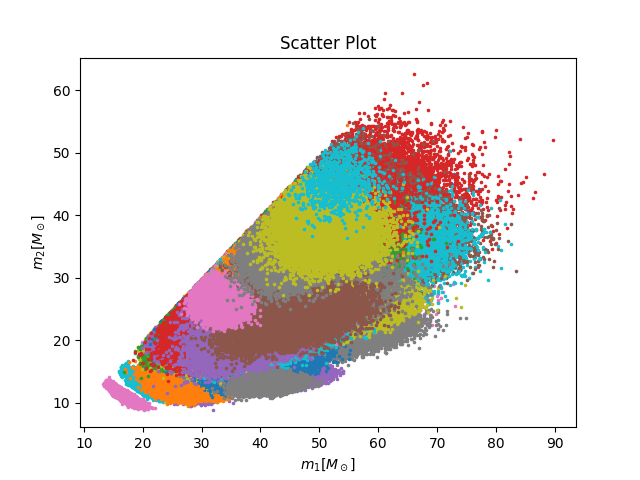
\includegraphics[width=0.49\textwidth]{figures/scatter_plot_10Hz.png}
    \caption{Comparison of the results with two different errors in $\beta$ calculations at $f=20 Hz$ (LHS) and $f=10 Hz$ (RHS).}
    \label{fig:fig1}
\end{figure}

The Fig. \ref{fig:fig2} show the comparison of the eccentric results with two different errors choosing $\beta$
calculations at $f=20 Hz$ and $f=10 Hz$.  The two results produce qualitatively similar results, except that the 10Hz
result (as required) inherits a larger mass uncertainty scale from the larger assumed zero-eccentricy chirp mass error
scale.

\begin{figure}[h]
    \centering
    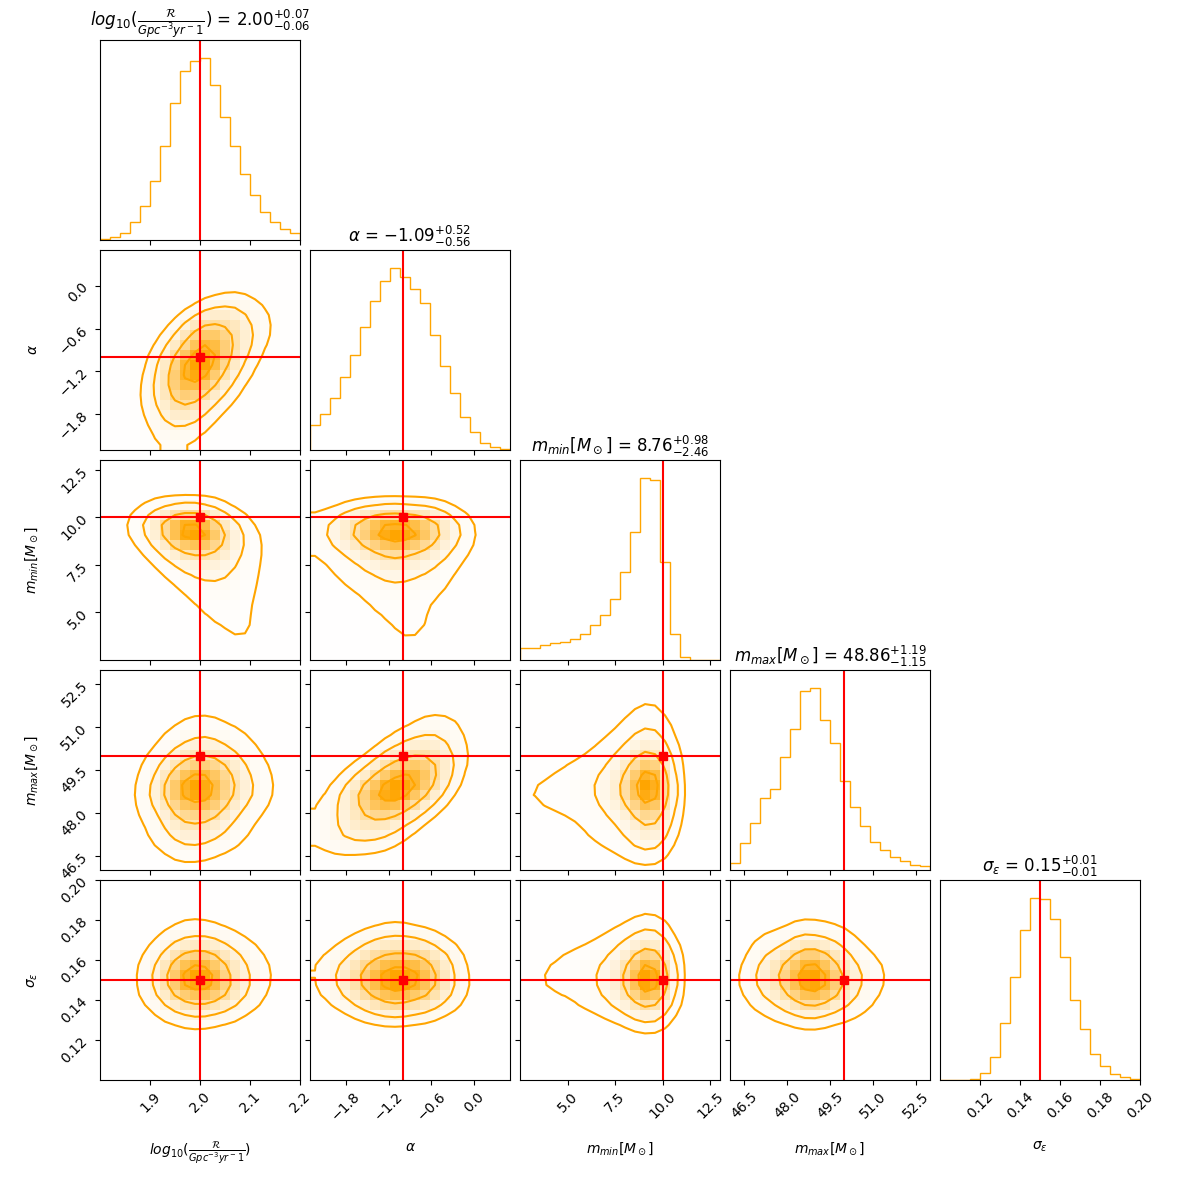
\includegraphics[width=0.49\textwidth]{figures/cor_ecc_015.png}
    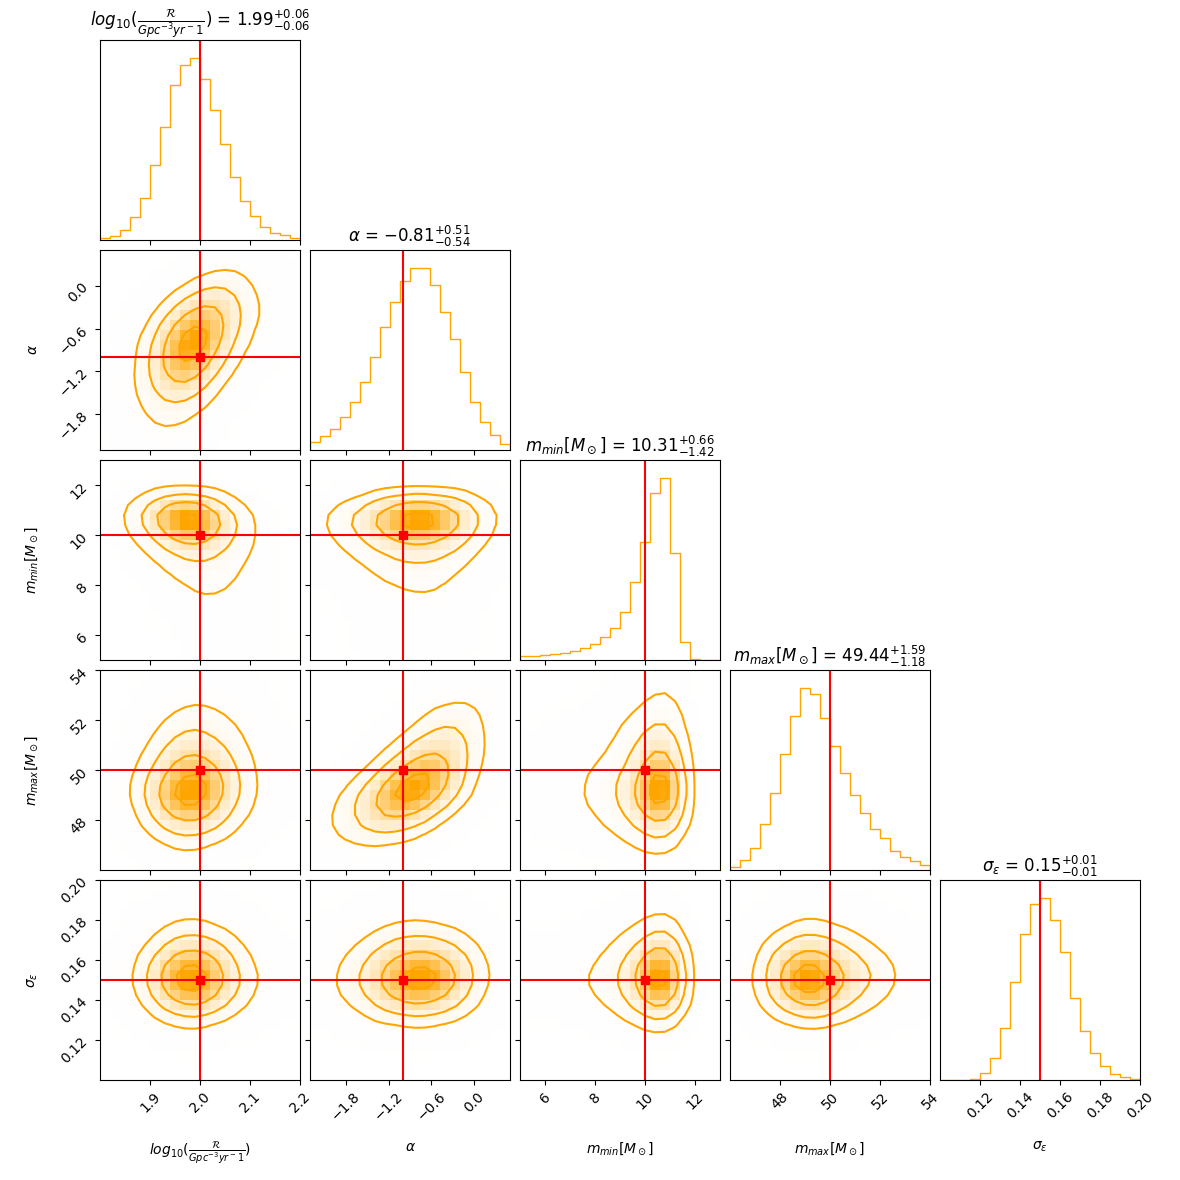
\includegraphics[width=0.49\textwidth]{figures/cor_ecc_015_10HZ.png}
    \caption{Comparison of the eccentric results with two different errors in $\beta$ calculations at $f=20 Hz$ (LHS) and $f=10 Hz$ (RHS).}
    \label{fig:fig2}
\end{figure}

The Fig. \ref{fig:fig3} are for the comparison between eccentric analyses (EBBH) and quasicircular analyses (CBBH) using
different choices for the assumed chirp mass uncertainty.  Again, the two results
are qualitatively similar, except that mass uncertainty scales are larger in the right side.

\begin{figure}[h]
    \centering
    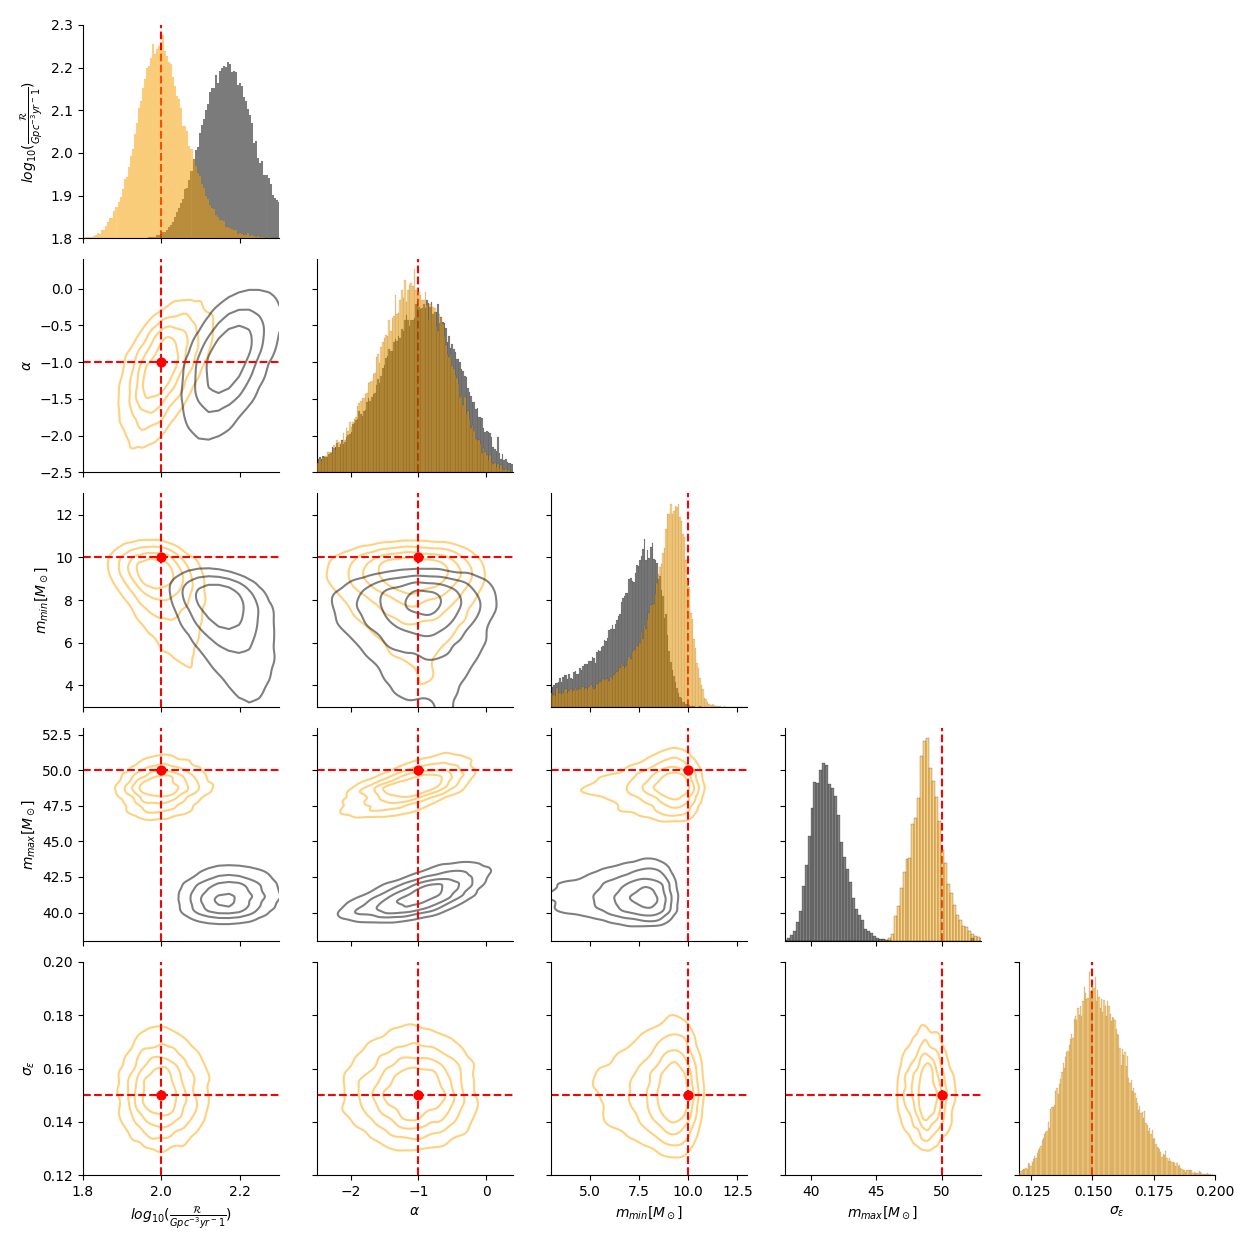
\includegraphics[width=0.49\textwidth]{figures/new_corner_015.png}
    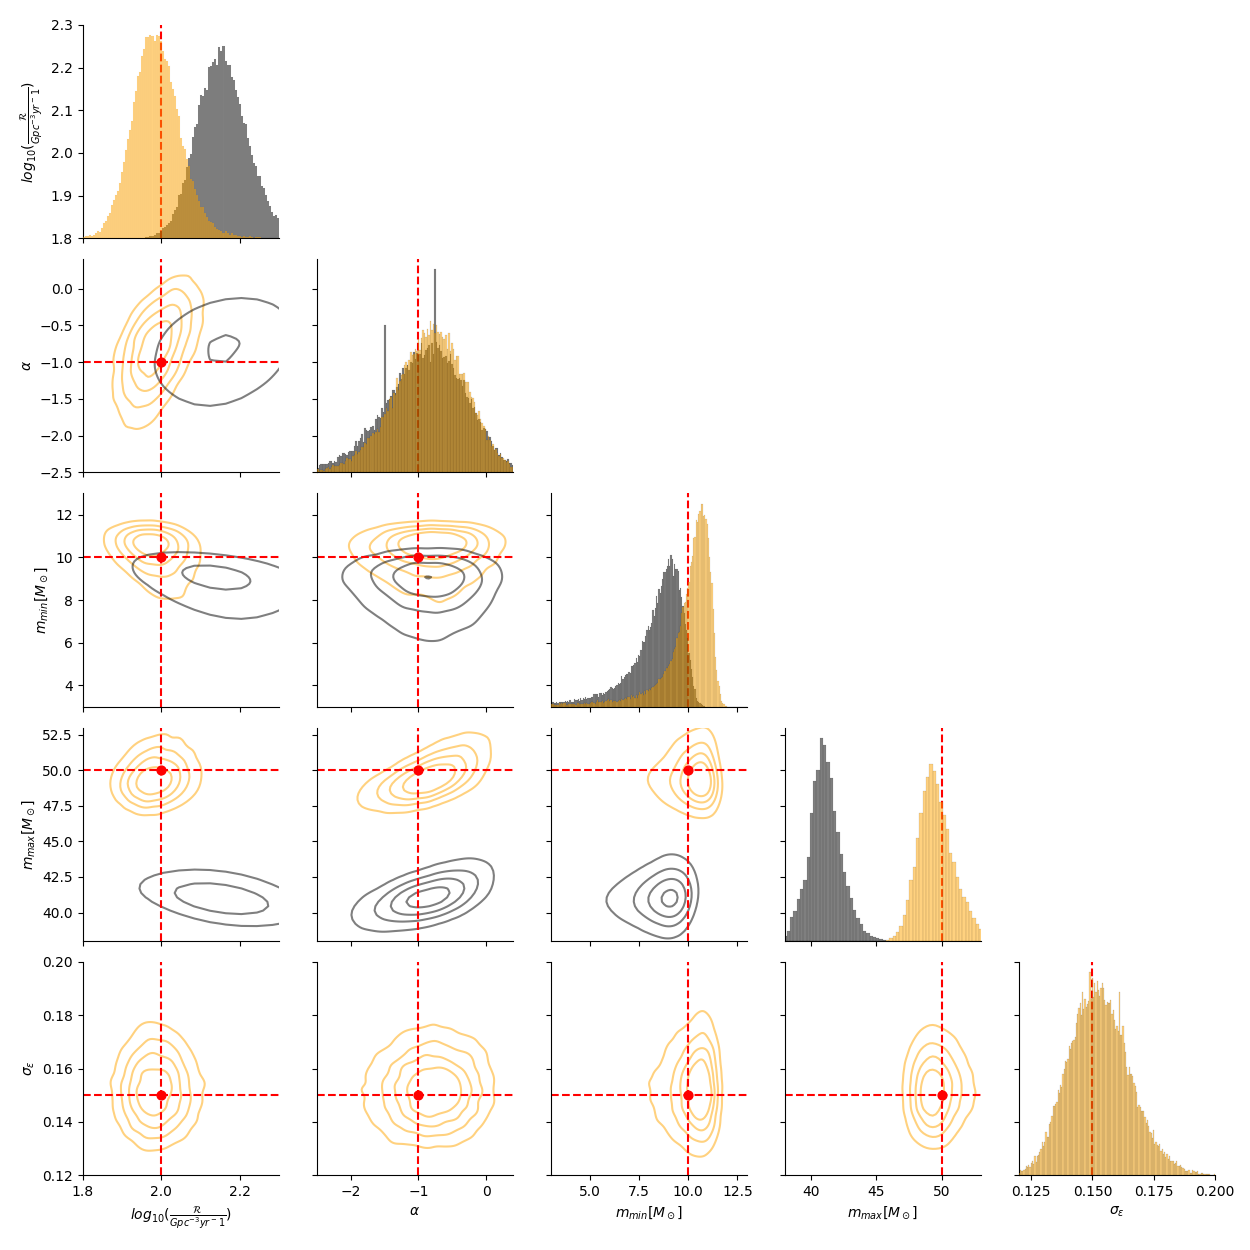
\includegraphics[width=0.49\textwidth]{figures/new_corner_015_10HZ.png}
    \caption{Comparison of the (EBBH (orange) and CBBH (black))results  with two different errors in $\beta$ calculations at $f=20 Hz$ (LHS) and $f=10 Hz$ (RHS).}
    \label{fig:fig3}
\end{figure}

\end{document}
